\chapter{Concentração e diluição}\label{ch:g10:concentration-and-dilution}

Uma bolsa de soro está pendurada acima da cama de um paciente. O rótulo
diz ``cloreto de sódio 0.9 \%'': sal na água, e mais nada. Mas o número
0.9 não é um detalhe. Com sal de menos, as células do sangue do paciente
incham de água; com sal demais, elas murcham. Uma solução não é descrita
só pelos seus ingredientes, mas por quanto \omterm{def:g6:solutions-and-solubility:solute}{soluto} cada volume dela
contém: a sua concentração. Este capítulo mede concentrações, prepara
soluções de concentração exata e as dilui.

\begin{recall}
Uma solução é formada por um \omterm{def:g6:solutions-and-solubility:solute}{solvente} e por um ou mais \omterm{def:g6:solutions-and-solubility:solute}{solutos}
dissolvidos; a \omterm{def:g6:solutions-and-solubility:solubility}{solubilidade} é a maior massa de \omterm{def:g6:solutions-and-solubility:solute}{soluto} que uma dada
quantidade de \omterm{def:g6:solutions-and-solubility:solute}{solvente} consegue \omterm{def:g2:mixing-and-dissolving:dissolve}{dissolver}
(\cref{ch:g6:solutions-and-solubility}). A \omterm{def:g10:the-mole:amount}{quantidade de matéria} de uma
espécie é $n = m/M$, em \omterm{def:g10:the-mole:amount}{mols} (\cref{ch:g10:the-mole}).
\end{recall}

\begin{omfigure}
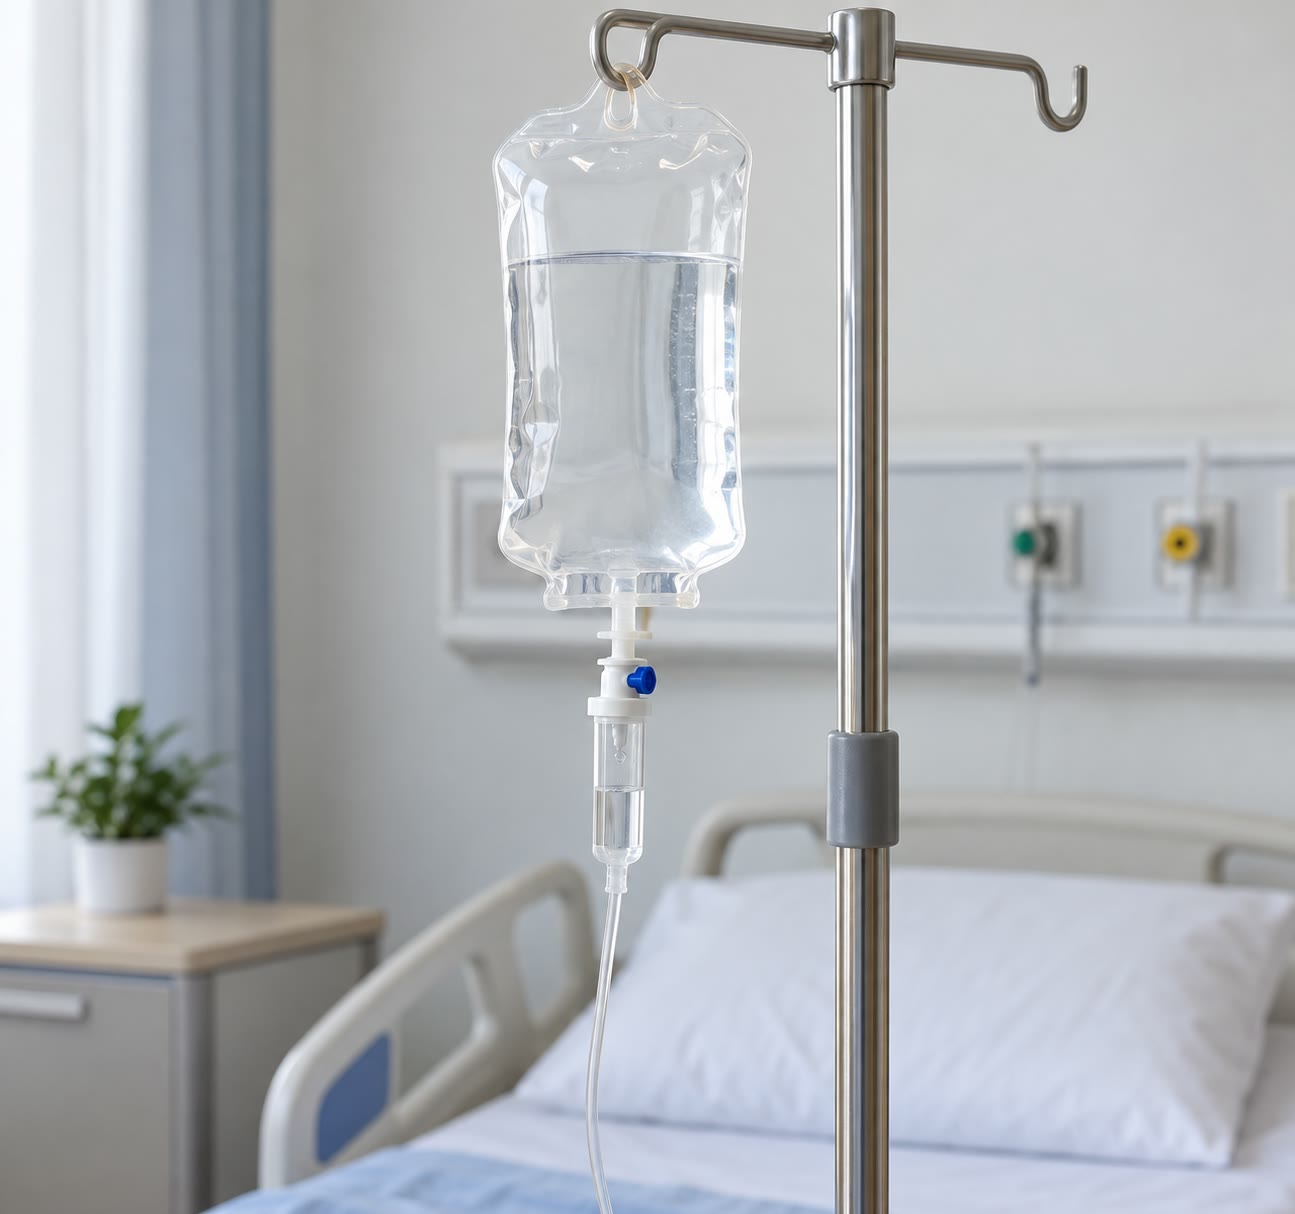
\includegraphics[width=0.42\linewidth]{images/book1/ai/g10-drip-bag.jpg}

{\small Uma bolsa de soro fisiológico: a concentração tem de estar
certa.}
\end{omfigure}

\section{A concentração em massa}

\begin{definition}[Concentração em massa]\label{def:g10:concentration-and-dilution:mass-concentration}
A \emph{concentração em massa}\index{concentracao em massa@concentração em massa} $C_m$ de um
\omterm{def:g6:solutions-and-solubility:solute}{soluto} numa solução é a massa de \omterm{def:g6:solutions-and-solubility:solute}{soluto} dissolvido por volume de
solução:
\[
  C_m = \frac{m_{\text{soluto}}}{V_{\text{solução}}},
\]
em gramas por litro (\si{g/L}).
\end{definition}

\begin{example}[Água com açúcar]\label{ex:g10:concentration-and-dilution:sugar}
Dissolvem-se \qty{20}{g} de açúcar em água, e a solução é completada até
\qty{0.50}{L}. A sua \omterm{def:g10:concentration-and-dilution:mass-concentration}{concentração em massa} de açúcar é
$C_m = \qty{20}{g} / \qty{0.50}{L} = \qty{40}{g/L}$. Qualquer parte dela
tem a mesma concentração: um copo de \qty{0.20}{L} dela contém
$\qty{40}{g/L} \times \qty{0.20}{L} = \qty{8.0}{g}$ de açúcar.
\end{example}


\begin{remark}[O volume é o da solução]\label{rem:g10:concentration-and-dilution:volume}
O volume em $C_m$ é o volume da solução inteira, e não o da água
despejada: \omterm{def:g2:mixing-and-dissolving:dissolve}{dissolver} um \omterm{def:g6:solutions-and-solubility:solute}{soluto} muda um pouco o volume. É por isso que
uma solução é sempre \emph{completada} até um volume final conhecido,
num frasco marcado para isso.
\end{remark}

\begin{remark}[Concentração não é solubilidade]\label{rem:g10:concentration-and-dilution:not-solubility}
% ledger: sol:NaCl, saline:NaCl
A \omterm{def:g6:solutions-and-solubility:solubility}{solubilidade} de um \omterm{def:g6:solutions-and-solubility:solute}{soluto} é a \emph{maior} concentração que ele pode
alcançar; uma solução pode ter qualquer concentração entre zero e esse
valor. O cloreto de sódio \omterm{def:g2:mixing-and-dissolving:dissolve}{se dissolve} até cerca de \qty{360}{g} por
quilograma de água a \qty{25}{\celsius}; a bolsa de soro só contém
\qty{9}{g} por litro, muito longe da saturação.
\end{remark}

\begin{remark}[As porcentagens dos rótulos]\label{rem:g10:concentration-and-dilution:percent}
% ledger: saline:NaCl
Nos rótulos de remédios e de alimentos, ``0.9 \%'' para um sólido
dissolvido em água em geral quer dizer \qty{0.9}{g} de \omterm{def:g6:solutions-and-solubility:solute}{soluto} por
\qty{100}{mL} de solução. Em gramas por litro, isso é dez vezes mais: a
bolsa de soro contém \qty{9.0}{g/L} de cloreto de sódio.
\end{remark}

\section{A concentração molar}

\begin{definition}[Concentração molar]\label{def:g10:concentration-and-dilution:molar-concentration}
A \emph{concentração molar}\index{concentracao molar@concentração molar} $c$ de um \omterm{def:g6:solutions-and-solubility:solute}{soluto}
numa solução, também chamada concentração em \omterm{def:g10:the-mole:amount}{quantidade de matéria}, é
a quantidade de \omterm{def:g6:solutions-and-solubility:solute}{soluto} dissolvido por volume de solução:
\[
  c = \frac{n_{\text{soluto}}}{V_{\text{solução}}},
\]
em \omterm{def:g10:the-mole:amount}{mols} por litro (\si{mol/L}).
\end{definition}

\begin{proposition}[De uma concentração à outra]\label{prop:g10:concentration-and-dilution:link}
Para um \omterm{def:g6:solutions-and-solubility:solute}{soluto} de \omterm{def:g10:the-mole:molar-mass}{massa molar} $M$,
\[
  C_m = c \times M .
\]
\end{proposition}

\begin{proof}
$C_m = m / V = (n \times M) / V = (n / V) \times M = c \times M$.
\end{proof}

\begin{example}[A bolsa de soro em mols]\label{ex:g10:concentration-and-dilution:drip}
% ledger: saline:NaCl, saline:Na, aw:Na, aw:Cl
A bolsa de soro contém \qty{9.0}{g/L} de cloreto de sódio, de \omterm{def:g10:the-mole:molar-mass}{massa
molar} \qty{58.5}{g/mol}. A sua \omterm{def:g10:concentration-and-dilution:molar-concentration}{concentração molar} é
\[
  c = \frac{C_m}{M} = \frac{\qty{9.0}{g/L}}{\qty{58.5}{g/mol}}
    = \qty{0.154}{mol/L}.
\]
O rótulo do fabricante dá o mesmo número pelo outro lado: 154 milésimos
de \omterm{def:g10:the-mole:amount}{mol} de \omterm{def:g9:ions:ion}{íons} sódio por litro.
\end{example}

\begin{remark}[Os íons em solução]\label{rem:g10:concentration-and-dilution:ions}
O cloreto de sódio \omterm{def:g2:mixing-and-dissolving:dissolve}{se dissolve} na forma de \omterm{def:g9:ions:ion}{íons} separados \ce{Na+} e
\ce{Cl-} (\cref{ch:g9:ions}): uma solução de cloreto de sódio a
\qty{0.154}{mol/L} contém \qty{0.154}{mol/L} de \omterm{def:g9:ions:ion}{íons} sódio e
\qty{0.154}{mol/L} de \omterm{def:g9:ions:ion}{íons} cloreto. Como um sólido iônico se desfaz na
água é o assunto de um capítulo mais adiante.
\end{remark}

\begin{omfigure}
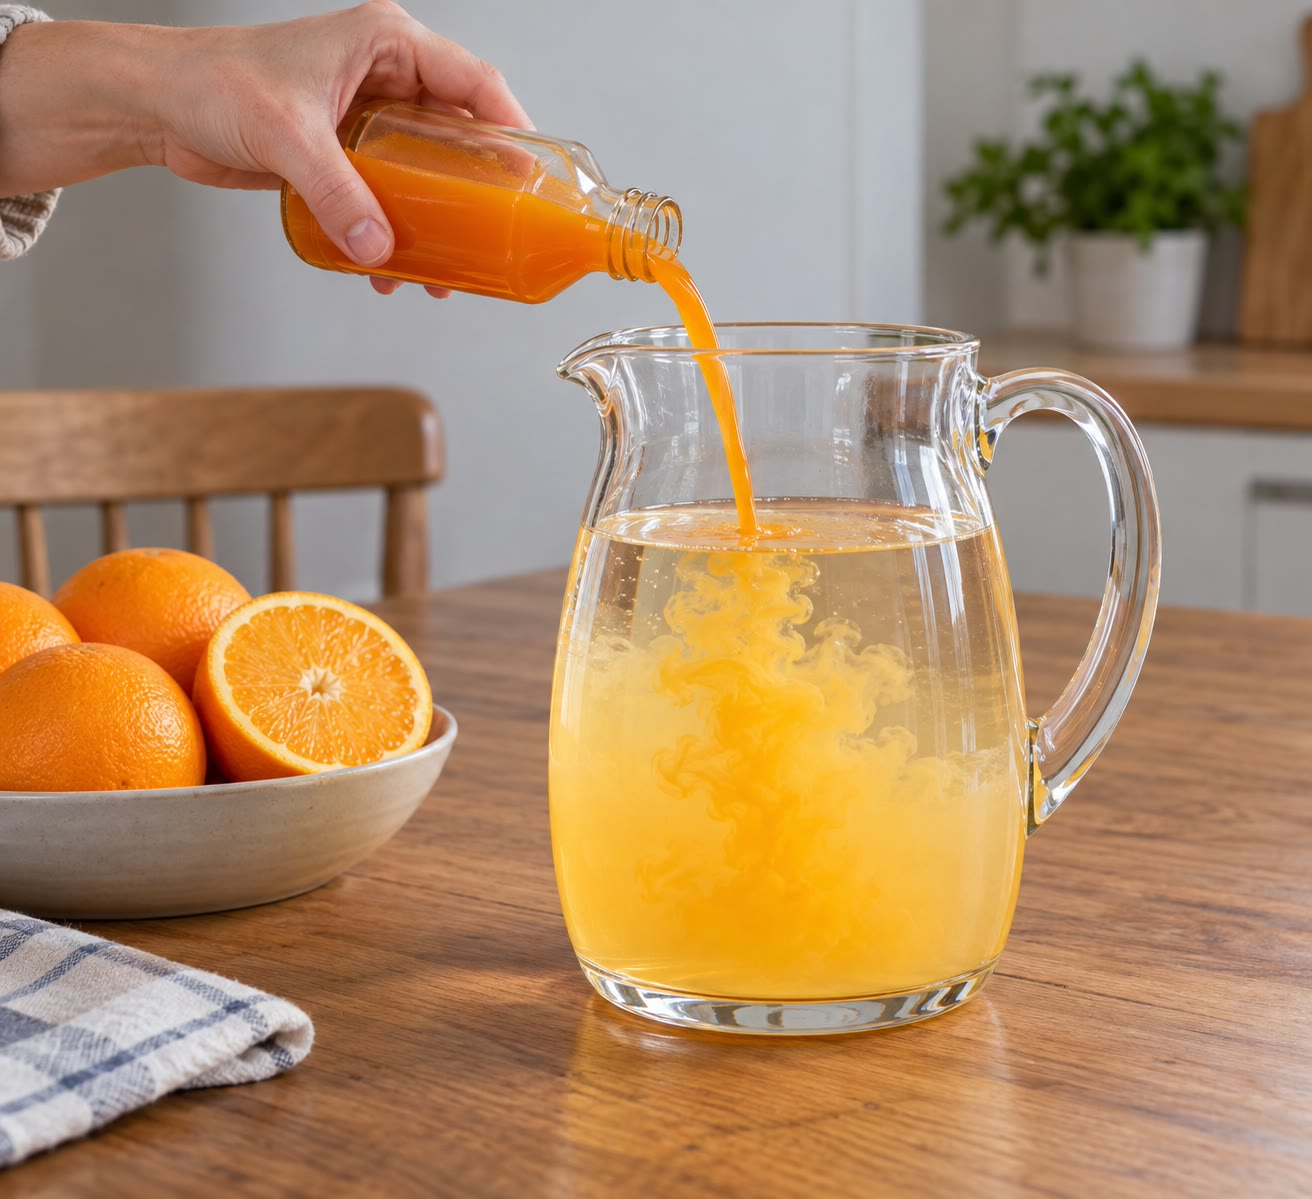
\includegraphics[width=0.45\linewidth]{images/book1/ai/g10-squash-jug.jpg}

{\small Um suco concentrado de garrafa é diluído com água numa jarra: a
bebida contém a mesma quantidade de xarope de fruta, num volume maior.}
\end{omfigure}

\section{Preparar uma solução por dissolução}

\begin{method}[Preparar uma solução dissolvendo um sólido]\label{met:g10:concentration-and-dilution:dissolving}
Para preparar um volume $V$ de solução de \omterm{def:g10:concentration-and-dilution:molar-concentration}{concentração molar} $c$:
\begin{enumerate}
  \item Calcule a quantidade necessária, $n = c \times V$, e a massa a
        pesar, $m = n \times M$.
  \item Pese essa massa de sólido num pequeno recipiente numa balança.
  \item Despeje o sólido, por um funil, num balão volumétrico de volume
        $V$; enxágue o recipiente e o funil com água destilada para
        dentro do balão, para que nenhum sólido se perca.
  \item Acrescente água destilada até cerca da metade do balão e agite
        em movimentos circulares até que todo o sólido se dissolva.
  \item Acrescente água destilada até a marca, as últimas gotas com um
        conta-gotas; tampe o balão e vire-o várias vezes para \omterm{def:g2:mixing-and-dissolving:mix}{misturar}.
\end{enumerate}
\end{method}

\begin{omfigure}
\begin{tikzpicture}[font=\small, scale=1.05]
  % 1. weigh
  \pic[transform shape] at (0,0) {balance};
  \fill[black!8, draw=black!55] (-0.45,0.8) -- (0.45,0.8) -- (0.38,0.98)
    -- (-0.38,0.98) -- cycle;
  \fill[white, draw=black!40] (-0.25,0.98) .. controls (-0.1,1.15) and
    (0.1,1.15) .. (0.25,0.98) -- cycle;
  \node[align=center, anchor=north] at (0,-0.2) {1. pese\\ o sólido};
  % 2. transfer through a funnel
  \pic[transform shape] at (3.2,0) {volflask={0.08}{omWater}};
  \pic[transform shape] at (3.2,3.0) {funnel};
  \draw[omProp, thick, -{Stealth}] (2.4,5.0) -- (2.85,4.65);
  \node[align=center, anchor=north] at (3.2,-0.2) {2. transfira,\\ enxágue};
  % 3. half full, swirl
  \pic[transform shape] at (6.4,0) {volflask={0.45}{omWater}};
  \draw[omProp, thick, -{Stealth}] (5.55,0.5) arc[start angle=200,
    end angle=340, x radius=0.9, y radius=0.3];
  \node[align=center, anchor=north] at (6.4,-0.2) {3. até a metade:\\ agite};
  % 4. to the mark
  \pic[transform shape] at (9.6,0) {volflask={1}{omWater}};
  \fill[black!45] (9.43,3.6) rectangle (9.77,3.85);
  \draw[omDef, thick, <-] (9.82,2.9) -- (10.6,3.3) node[right] {marca};
  \node[align=center, anchor=north] at (9.6,-0.2) {4. até a marca,\\
    tampe, misture};
\end{tikzpicture}

{\small Preparar uma solução dissolvendo um sólido: pesar, transferir,
\omterm{def:g2:mixing-and-dissolving:dissolve}{dissolver} e completar até a marca do balão volumétrico.}
\end{omfigure}

\begin{inthelab}[Completar até a marca]
A marca de um balão volumétrico é um anel em volta do gargalo. A água
num tubo de vidro estreito não termina plana: a sua superfície se curva
para baixo no meio, formando um menisco. O balão está cheio quando a
\emph{parte de baixo} do menisco toca a marca, vista com o olho na altura
da marca, de modo que a frente e o fundo do anel pareçam uma única
linha. Visto de cima ou de baixo, o nível pode parecer certo quando não
está.
\end{inthelab}

\begin{omfigure}
\begin{tikzpicture}[font=\small]
  \newcommand{\neck}[2]{% x, meniscus bottom height
    \fill[omWater] (#1-0.5,0) -- (#1-0.5,{#2+0.25}) .. controls
      (#1-0.25,#2) and (#1+0.25,#2) .. (#1+0.5,{#2+0.25}) -- (#1+0.5,0) -- cycle;
    \draw[black!60, line width=0.8pt] (#1-0.5,0) -- (#1-0.5,3);
    \draw[black!60, line width=0.8pt] (#1+0.5,0) -- (#1+0.5,3);
    \draw[omDef, line width=0.9pt] (#1-0.5,1.5) -- (#1+0.5,1.5);
    \draw[black!50] (#1-0.5,{#2+0.25}) .. controls (#1-0.25,#2) and
      (#1+0.25,#2) .. (#1+0.5,{#2+0.25});}
  \newcommand{\eye}[2]{% x, y: an eye looking to the right
    \draw[black!70] (#1-0.25,#2) .. controls (#1-0.1,#2+0.18) and
      (#1+0.1,#2+0.18) .. (#1+0.2,#2) .. controls (#1+0.1,#2-0.18) and
      (#1-0.1,#2-0.18) .. (#1-0.25,#2);
    \fill[black!70] (#1+0.05,#2) circle (0.06);}
  % right
  \neck{1.5}{1.5}
  \eye{-0.4}{1.5}
  \draw[dashed, black!50] (-0.1,1.5) -- (2.4,1.5);
  \node[align=center] at (1.5,-0.55) {certo: olho na altura,\\ fundo na marca};
  % too high
  \neck{6}{1.85}
  \eye{4.1}{1.85}
  \draw[dashed, black!50] (4.4,1.85) -- (6.9,1.85);
  \node[align=center] at (6,-0.55) {água demais:\\ menisco acima};
  % too low
  \neck{10.5}{0.85}
  \eye{8.6}{0.85}
  \draw[dashed, black!50] (8.9,0.85) -- (11.4,0.85);
  \node[align=center] at (10.5,-0.55) {água de menos:\\ menisco abaixo};
\end{tikzpicture}

{\small O gargalo de um balão volumétrico, ampliado e visto com o olho
na altura do menisco. A linha azul é a marca. Só o balão da esquerda
está corretamente cheio.}
\end{omfigure}

\section{Diluir}

\begin{definition}[Diluição, solução-estoque, fator de diluição]\label{def:g10:concentration-and-dilution:dilution}
Uma \emph{diluição}\index{diluicao@diluição} diminui a concentração de uma
solução por acréscimo de \omterm{def:g6:solutions-and-solubility:solute}{solvente}. A solução concentrada tomada no
início é a \emph{solução-estoque}\index{solucao-estoque@solução-estoque}. O \emph{fator
de diluição}\index{fator de diluicao@fator de diluição} $F$ é a razão entre a
concentração da solução-estoque e a da solução diluída:
\[
  F = \frac{c_{\text{estoque}}}{c_{\text{diluída}}} .
\]
\end{definition}

\begin{proposition}[A quantidade de soluto se conserva]\label{prop:g10:concentration-and-dilution:kept}
Durante uma \omterm{def:g10:concentration-and-dilution:dilution}{diluição}, a quantidade de \omterm{def:g6:solutions-and-solubility:solute}{soluto} não muda: se um volume
$V_0$ de \omterm{def:g10:concentration-and-dilution:dilution}{solução-estoque} de concentração $c_0$ for completado até um
volume $V_1$, a solução diluída tem a concentração $c_1$ dada por
\[
  c_0 \times V_0 = c_1 \times V_1,
  \qquad\text{logo}\qquad
  F = \frac{c_0}{c_1} = \frac{V_1}{V_0} .
\]
O mesmo vale para as \omterm{def:g10:concentration-and-dilution:mass-concentration}{concentrações em massa}.
\end{proposition}

\begin{proof}
Só se acrescenta \omterm{def:g6:solutions-and-solubility:solute}{solvente}: o \omterm{def:g6:solutions-and-solubility:solute}{soluto} tomado com o volume $V_0$, uma
quantidade $c_0 V_0$, está todo no volume final $V_1$, onde ele forma a
quantidade $c_1 V_1$.
\end{proof}


\begin{method}[Preparar uma solução por diluição]\label{met:g10:concentration-and-dilution:diluting}
Para preparar um volume $V_1$ de solução de concentração $c_1$ a partir
de uma \omterm{def:g10:concentration-and-dilution:dilution}{solução-estoque} de concentração $c_0$:
\begin{enumerate}
  \item Calcule o volume de \omterm{def:g10:concentration-and-dilution:dilution}{solução-estoque} a tomar,
        $V_0 = c_1 V_1 / c_0$ (isto é, $V_1 / F$).
  \item Despeje um pouco de \omterm{def:g10:concentration-and-dilution:dilution}{solução-estoque} num béquer limpo (nunca
        pipete direto do frasco) e tome exatamente $V_0$ com uma pipeta
        volumétrica, cheia até a sua marca.
  \item Deixe a pipeta escoar num balão volumétrico de volume $V_1$.
  \item Acrescente água destilada até a marca, tampe e \omterm{def:g2:mixing-and-dissolving:mix}{misture}.
\end{enumerate}
\end{method}

\begin{example}[Uma diluição de dez vezes]\label{ex:g10:concentration-and-dilution:tenfold}
Uma \omterm{def:g10:concentration-and-dilution:dilution}{solução-estoque} de sulfato de cobre tem $c_0 = \qty{0.10}{mol/L}$;
são necessários \qty{100.0}{mL} a $c_1 = \qty{0.010}{mol/L}$. O \omterm{def:g10:concentration-and-dilution:dilution}{fator de
diluição} é $F = 0.10 / 0.010 = 10$, logo $V_0 = \qty{100.0}{mL} / 10 =
\qty{10.0}{mL}$: uma pipeta de \qty{10.0}{mL} e um balão de
\qty{100.0}{mL}.
\end{example}

\begin{omfigure}
\begin{tikzpicture}[font=\small, scale=0.85]
  % 1. take the stock with a pipette
  \pic[transform shape] at (0,0) {beaker={0.6}{cyan!70!blue!55}};
  \pic[transform shape] at (0,0.2) {pipette={1}{cyan!70!blue!55}};
  \node[align=center, anchor=north] at (0,-0.2) {1. pipete $V_0$\\ da solução-estoque};
  \draw[omProp, very thick, -{Stealth}] (1.3,2.6) -- (2.6,2.6);
  % 2. empty it into the flask
  \pic[transform shape] at (4,0) {volflask={0.22}{cyan!70!blue!55}};
  \pic[transform shape] at (4,2.6) {pipette={0.12}{cyan!70!blue!55}};
  \node[align=center, anchor=north] at (4,-0.2) {2. esvazie-a\\ no balão};
  \draw[omProp, very thick, -{Stealth}] (5.3,2.6) -- (6.6,2.6);
  % 3. water to the mark
  \pic[transform shape] at (8,0) {volflask={1}{cyan!70!blue!14}};
  \draw[omDef, thick, <-] (8.2,2.9) -- (9.1,3.4) node[right] {marca};
  \node[align=center, anchor=north] at (8,-0.2) {3. água até a marca:\\
    volume $V_1$};
\end{tikzpicture}

{\small Diluir: um volume $V_0$ de \omterm{def:g10:concentration-and-dilution:dilution}{solução-estoque}, medido com uma
pipeta, é completado até $V_1$ num balão volumétrico. A cor fica mais
fraca na proporção do \omterm{def:g10:concentration-and-dilution:dilution}{fator de diluição} $V_1 / V_0$.}
\end{omfigure}

\section{Uma escala de padrões}

\begin{definition}[Solução-padrão, escala de padrões]\label{def:g10:concentration-and-dilution:standard}
Uma \emph{solução-padrão}\index{solucao-padrao@solução-padrão} é uma solução cuja
concentração é conhecida com exatidão. Uma \emph{escala de
padrões}\index{escala de padroes@escala de padrões} é uma série de soluções-padrão do
mesmo \omterm{def:g6:solutions-and-solubility:solute}{soluto}, em concentrações crescentes, em geral preparadas diluindo
uma mesma \omterm{def:g10:concentration-and-dilution:dilution}{solução-estoque}; comparar uma solução desconhecida com ela dá
uma estimativa da concentração da desconhecida.
\end{definition}

\begin{example}[Uma escala azul]\label{ex:g10:concentration-and-dilution:scale}
A partir de uma \omterm{def:g10:concentration-and-dilution:dilution}{solução-estoque} de sulfato de cobre a \qty{0.20}{mol/L},
preparam-se seis padrões a 0.02, 0.04, 0.06, 0.08, 0.10 e
\qty{0.12}{mol/L}, cada um em tubos idênticos cheios até a mesma altura.
Uma solução de concentração desconhecida, no mesmo tipo de tubo, parece
mais escura que o tubo de \qty{0.06}{mol/L} e mais clara que o de
\qty{0.08}{mol/L}: a sua concentração fica entre as duas, cerca de
\qty{0.07}{mol/L}.
\end{example}

\begin{omfigure}
\begin{tikzpicture}[font=\small]
  \foreach \i/\c/\p in {0/0.02/8, 1/0.04/16, 2/0.06/24, 3/0.08/32,
                        4/0.10/40, 5/0.12/48} {
    \pic at (1.2*\i,0) {testtube={0.75}{cyan!70!blue!\p}};
    \node[anchor=north] at (1.2*\i,-0.15) {\c};
  }
  \pic at (8.4,0) {testtube={0.75}{cyan!70!blue!28}};
  \node[anchor=north] at (8.4,-0.15) {?};
  \draw[black!40] (7.55,-0.6) -- (7.55,3.2);
  \node[anchor=north] at (3,-0.7) {concentração (\si{mol/L})};
  \node[anchor=north] at (8.4,-0.7) {desconhecida};
\end{tikzpicture}

{\small Uma \omterm{def:g10:concentration-and-dilution:standard}{escala de padrões} de soluções de sulfato de cobre e uma
solução desconhecida. A desconhecida fica entre o terceiro e o quarto
tubos.}
\end{omfigure}

\begin{safety}{\ghs[0.82cm]{GHS05}\ghs[0.82cm]{GHS07}\ghs[0.82cm]{GHS09}}
% ledger: ghs:CuSO4
Soluções de sulfato de cobre: nocivas se ingeridas, irritantes para a
pele, lesivas para os olhos, muito tóxicas para os organismos aquáticos.
Óculos de proteção e luvas; as soluções usadas são recolhidas para
tratamento, nunca jogadas na pia.
\end{safety}

\begin{remark}[Os limites do olho]\label{rem:g10:concentration-and-dilution:eye}
O olho só consegue dizer ``entre estes dois tubos''. Para medir uma
concentração com mais precisão a partir da cor de uma solução, os
químicos medem quanta luz ela absorve; um capítulo mais adiante faz
exatamente isso.
\end{remark}

\section{Exercícios}

\begin{exercise}[$\star$]\label{exo:g10:concentration-and-dilution:1}
Dissolvem-se \qty{5.0}{g} de açúcar para fazer \qty{250}{mL} de solução.
Calcule a \omterm{def:g10:concentration-and-dilution:mass-concentration}{concentração em massa} de açúcar, em gramas por litro.
\end{exercise}

\begin{exercise}[$\star$]\label{exo:g10:concentration-and-dilution:2}
Uma solução de \qty{200}{mL} contém \qty{0.050}{mol} de glicose. Calcule
a sua \omterm{def:g10:concentration-and-dilution:molar-concentration}{concentração molar}.
\end{exercise}

\begin{exercise}[$\star$]\label{exo:g10:concentration-and-dilution:3}
Que massa de sulfato de cobre anidro \ce{CuSO4} deve ser pesada para
preparar \qty{100.0}{mL} de solução a \qty{0.10}{mol/L}?
\end{exercise}

\begin{exercise}[$\star$]\label{exo:g10:concentration-and-dilution:4}
Uma \omterm{def:g10:concentration-and-dilution:dilution}{solução-estoque} a \qty{1.0}{mol/L} é diluída até \qty{0.050}{mol/L}.
Qual é o \omterm{def:g10:concentration-and-dilution:dilution}{fator de diluição}? Que volume de \omterm{def:g10:concentration-and-dilution:dilution}{solução-estoque} é necessário
para fazer \qty{100.0}{mL} de solução diluída?
\end{exercise}

\begin{exercise}[$\star$]\label{exo:g10:concentration-and-dilution:5}
Uma solução de cloreto de sódio tem \omterm{def:g10:concentration-and-dilution:molar-concentration}{concentração molar} de
\qty{0.10}{mol/L}. Qual é a sua \omterm{def:g10:concentration-and-dilution:mass-concentration}{concentração em massa}?
\end{exercise}

\begin{exercise}[$\star\star$]\label{exo:g10:concentration-and-dilution:6}
Que volume de uma \omterm{def:g10:concentration-and-dilution:dilution}{solução-estoque} a \qty{0.50}{mol/L} deve ser tomado
para preparar \qty{250.0}{mL} de solução a \qty{0.020}{mol/L}? Dê o nome
das duas vidrarias usadas.
\end{exercise}

\begin{exercise}[$\star\star$]\label{exo:g10:concentration-and-dilution:7}
Por que uma solução de concentração exata é preparada num balão
volumétrico, e não num béquer graduado? Por que um volume de
\omterm{def:g10:concentration-and-dilution:dilution}{solução-estoque} é medido com uma pipeta volumétrica, e não com uma
proveta?
\end{exercise}

\begin{exercise}[$\star\star$]\label{exo:g10:concentration-and-dilution:8}
Olhe a \omterm{def:g10:concentration-and-dilution:standard}{escala de padrões} de sulfato de cobre. Uma segunda solução
desconhecida é mais clara que o tubo de \qty{0.04}{mol/L}, mas mais
escura que o de \qty{0.02}{mol/L}. Estime a sua concentração. Como a
escala poderia ser mudada para estimá-la com mais precisão?
\end{exercise}

\begin{exercise}[$\star\star$]\label{exo:g10:concentration-and-dilution:9}
Uma solução de glicose para infusão contém \qty{50}{g/L} de glicose
\ce{C6H12O6}. Calcule a sua \omterm{def:g10:concentration-and-dilution:molar-concentration}{concentração molar}.
\end{exercise}

\begin{exercise}[$\star\star$]\label{exo:g10:concentration-and-dilution:10}
Um xarope é feito dissolvendo \qty{342}{g} de sacarose \ce{C12H22O11}
para obter \qty{1.00}{L} de solução. Calcule a sua \omterm{def:g10:concentration-and-dilution:molar-concentration}{concentração molar}.
Ele é depois diluído dez vezes. Que massa de sacarose contém uma
colherada de \qty{20}{mL} do xarope diluído?
\end{exercise}

\begin{exercise}[$\star\star$]\label{exo:g10:concentration-and-dilution:11}
Uma solução tem \omterm{def:g10:concentration-and-dilution:mass-concentration}{concentração em massa} de \qty{12}{g/L}. Qual é a sua
concentração (a) depois que se acrescenta água para dobrar o seu volume;
(b) depois que metade da sua água \omterm{def:g3:separating-mixtures:evaporate}{evaporou}, com todo o \omterm{def:g6:solutions-and-solubility:solute}{soluto}
continuando dissolvido?
\end{exercise}

\begin{exercise}[$\star\star\star$]\label{exo:g10:concentration-and-dilution:12}
Uma solução a \qty{0.10}{mol/L} é diluída dez vezes, o resultado é
diluído dez vezes de novo, e mais uma vez.
\begin{enumerate}
  \item Qual é a concentração final?
  \item Por que isso é feito em três etapas, e não numa única \omterm{def:g10:concentration-and-dilution:dilution}{diluição}
        de 1000 vezes (pense nos volumes das vidrarias necessárias)?
\end{enumerate}
\end{exercise}

\begin{exercise}[$\star\star\star$]\label{exo:g10:concentration-and-dilution:13}
Dissolvem-se \qty{11.1}{g} de cloreto de cálcio \ce{CaCl2} para fazer
\qty{500.0}{mL} de solução. Na água, o sólido se separa em \omterm{def:g9:ions:ion}{íons} cálcio
\ce{Ca^2+} e \omterm{def:g9:ions:ion}{íons} cloreto \ce{Cl-}.
\begin{enumerate}
  \item Calcule a \omterm{def:g10:concentration-and-dilution:molar-concentration}{concentração molar} de cloreto de cálcio dissolvido.
  \item Deduza as \omterm{def:g10:concentration-and-dilution:molar-concentration}{concentrações molares} dos \omterm{def:g9:ions:ion}{íons} cálcio e dos \omterm{def:g9:ions:ion}{íons}
        cloreto na solução.
\end{enumerate}
\end{exercise}

\begin{exercise}[$\star\star\star$]\label{exo:g10:concentration-and-dilution:14}
Um balão volumétrico de \qty{100.0}{mL} tem um gargalo de diâmetro
interno \qty{1.2}{cm}. Um aluno o enche com a parte de baixo do menisco
\qty{2}{mm} acima da marca.
\begin{enumerate}
  \item Que volume de água a mais foi acrescentado (volume de um
        cilindro: $\pi r^2 h$)?
  \item Em que porcentagem a concentração da solução fica baixa demais?
\end{enumerate}
\end{exercise}

\begin{exercise}[$\star\star\star$]\label{exo:g10:concentration-and-dilution:15}
Misturam-se \qty{100}{mL} de solução de cloreto de sódio a
\qty{0.20}{mol/L} com \qty{300}{mL} de solução de cloreto de sódio a
\qty{0.10}{mol/L}. Supondo que os volumes se somam, calcule a
concentração da \omterm{def:g6:pure-substances-and-mixtures:mixture}{mistura}. Ela é a média das duas concentrações?
Explique.
\end{exercise}

\section{Problema: a bolsa de soro}

\begin{problem}[{Problema de fim de semana --- quanto de uma solução
salina concentrada vai para uma bolsa de soro ``0.9 \%''?}]
\label{pb:g10:concentration-and-dilution:1}
% ledger: saline:NaCl, saline:Na, sol:NaCl, aw:Na, aw:Cl, const:NA
O laboratório da farmácia de um hospital guarda uma solução estéril
concentrada de cloreto de sódio com \qty{200}{g/L} (no rótulo: ``20
\%''). Ele precisa preparar bolsas de \qty{500}{mL} da solução ``0.9 \%''
usada nas infusões, diluindo a solução concentrada com água estéril.

\medskip
\noindent\textbf{Parte I --- O que quer dizer 0.9 \%.}
\begin{enumerate}
  \item O rótulo ``0.9 \%'' quer dizer \qty{0.9}{g} de sal por
        \qty{100}{mL} de solução. Dê a \omterm{def:g10:concentration-and-dilution:mass-concentration}{concentração em massa} em
        \si{g/L}.
  \item Expresse-a também em miligramas por mililitro.
  \item Que massa de cloreto de sódio contém uma bolsa de
        \qty{500}{mL}?
  \item O cloreto de sódio \omterm{def:g2:mixing-and-dissolving:dissolve}{se dissolve} até cerca de \qty{360}{g} por
        quilograma de água. A solução da bolsa está longe da saturação?
  \item Um paciente recebe \qty{1.0}{L} dessa solução num dia. Que massa
        de sal é essa?
\end{enumerate}

\medskip
\noindent\textbf{Parte II --- Em \omterm{def:g10:the-mole:amount}{mols}.}
\begin{enumerate}[resume]
  \item Calcule a \omterm{def:g10:the-mole:molar-mass}{massa molar} do cloreto de sódio.
  \item Calcule a \omterm{def:g10:concentration-and-dilution:molar-concentration}{concentração molar} da solução da bolsa.
  \item Que quantidade de cloreto de sódio uma bolsa contém?
  \item Quais são as \omterm{def:g10:concentration-and-dilution:molar-concentration}{concentrações molares} dos \omterm{def:g9:ions:ion}{íons} sódio e dos \omterm{def:g9:ions:ion}{íons}
        cloreto na bolsa?
  \item Quantos \omterm{def:g9:ions:ion}{íons} sódio uma bolsa contém?
\end{enumerate}

\medskip
\noindent\textbf{Parte III --- A partir da solução concentrada.}
\begin{enumerate}[resume]
  \item Calcule o \omterm{def:g10:concentration-and-dilution:dilution}{fator de diluição} entre a solução concentrada e a
        solução da bolsa.
  \item Que massa de cloreto de sódio deve vir da solução concentrada
        para uma bolsa? Deduza o volume de solução concentrada a tomar.
  \item Confira esse volume com o \omterm{def:g10:concentration-and-dilution:dilution}{fator de diluição}.
  \item Calcule a \omterm{def:g10:concentration-and-dilution:molar-concentration}{concentração molar} da solução concentrada, e
        verifique que $c_0 V_0 = c_1 V_1$.
  \item Mais ou menos que volume de água estéril é acrescentado então
        (suponha que os volumes se somam)?
\end{enumerate}

\medskip
\noindent\textbf{Parte IV --- Vidraria e exatidão.}
\begin{enumerate}[resume]
  \item Não existe pipeta volumétrica desse volume. Que vidraria,
        graduada em décimos de mililitro, poderia fornecê-lo?
  \item Em que recipiente o volume final deve ser completado, para ser
        exato?
  \item Se fossem tomados \qty{23.0}{mL} em vez do volume certo, que
        \omterm{def:g10:concentration-and-dilution:mass-concentration}{concentração em massa} a bolsa teria? Em que porcentagem ela
        estaria errada?
  \item Dê a resposta final: que volume da solução concentrada vai para
        uma bolsa de \qty{500}{mL}?
\end{enumerate}
\end{problem}
